\documentclass[14pt,a4paper]{extarticle}
%\documentclass[12pt,a4paper]{article}

\usepackage[utf8]{inputenc}
\usepackage[ukrainian]{babel}


\usepackage{amssymb}
\usepackage{physics}
\usepackage{dsfont}

\usepackage[active]{srcltx}
\usepackage[final]{pdfpages}

\usepackage[hidelinks]{hyperref}

\usepackage{verbatim}
%%%%%%%%%%%%%%%%%%%%%%%%%%%%%%%%%%%%%%%%%%%%%%%%%%%%%%%%%%%%%%%%%%
%\pagestyle{empty}                     %нумерацiя сторiнок i т.д.
\pagestyle{headings}                   %нумерацiя сторiнок вгорi зправа i т.д.
%\renewcommand{\baselinestretch}{1.5}   %мiжстрiчковий інтервал
%\parindent=7.5mm                      %абзацний відступ
 \righthyphenmin=2                     %перенос 2 останніх букв
 \pagenumbering{arabic}
 \tolerance=400
 \mathsurround=2pt
 \hfuzz=1.5pt
%%%%%%%%%%%%%%%%%%%%%%%%%%%%%%%%%%%%%%%%%%%%%%%%%%%%%%%%%%%%%%%%%%
 %\hoffset=-0.5cm        %+2.5cm -- вiдступ вiд лiвого краю
 %\voffset=-1.5cm        %+2.5cm -- вiдступ зверху
 %\oddsidemargin=0.1cm   %ліве поле
 %\topmargin=0.1cm       %верхнє поле
 %\headheight=0.5cm      %висота верхнього колонтитулу
 %\footskip=1cm          %висота нижнього колонтитулу
 %\headsep=0.3cm         %відступ від колонт. до тексту
 %\textwidth=17cm        %ширина сторінки
 %\textheight=25.5cm     %висота сторінки

\usepackage{kantlipsum}

\pdfpageheight=297mm
\pdfpagewidth=210mm
\pdfhorigin=\dimexpr1in+(210mm-8.5in)/2\relax
\pdfvorigin=\dimexpr1in+(297mm-11in)/2\relax

\usepackage{geometry}
\geometry{
    a4paper,
    total={175mm,252mm},
    left=30mm,
    top=15mm,
    right=10mm,
    bottom=20mm,
}

 \renewcommand{\baselinestretch}{1.5}
%%%%%%%%%%%%%%%%%%%%%%%%%%%%%%%%%%%%%%%%%%%%%%%%%%%%%%%%%%%%%%%%%%
 \newcounter{e}
 \setcounter{e}{0}
 \newcommand{\n}{\refstepcounter{e} (\arabic{e})}
 
 \newcounter{pic}
 \setcounter{pic}{0}
 \newcommand{\pic}[1]{\refstepcounter{pic} \vspace{-0.3cm}\textit{Figure \arabic{pic}\label{#1}.}}
 
 \newcounter{tabl}
 \setcounter{tabl}{0}
 \newcommand{\tabl}[1]{\refstepcounter{tabl} \vspace{-0.3cm}\textit{Table \arabic{tabl}\label{#1}.}}
 
 \newcounter{dod}
 \setcounter{dod}{0}
 \newcommand{\dod}[1]{\refstepcounter{dod} \textit{Appendix \arabic{dod}\label{#1}.}}
 
% \newcounter{defn}
 %\setcounter{defn}{0}
 %\newcommand{\defn}[1]{\refstepcounter{defn} %\textbf{Означення \arabic{defn}\label{#1}.}}
 
 %\newcounter{theorem}
 %\setcounter{theorem}{0}
 %\newcommand{\theorem}[1]{\refstepcounter{theorem} %\textbf{Теорема \arabic{theorem}\label{#1}.}}
 \newtheorem{theorem}{Theorem}[section]
 \newtheorem{defn}[theorem]{Definition}
 \newtheorem{lemma}[theorem]{Lemma}
 
 \newcommand{\proof}{\textit{Proof. \space}}
% \setcounter{page}{1}
% \setcounter{section}{1}

\numberwithin{equation}{section}
\numberwithin{figure}{section}
%%%%%%%%%%%%%%%%%%%%%%%%%%%%%%%%%%%%%%%%%%%%%%%%%%%%%%%%%%%%%%%%%%
 \newcounter{stali}
 \setcounter{stali}{0}
 \newcommand{\s}{\refstepcounter{stali} \arabic{stali}}

 \newcommand{\st}{C_{\s}}
 \newcommand{\stl}[1]{C_{\s \label{#1}}}

 \newcommand{\cd}{{} $$ \vspace{-0.3cm} $$ {}}
 
 \newcommand{\nb}[2]{\righthyphenmin=#2 #1 \righthyphenmin=2}

%%%%%%%%%%%%%%%%%%%%%%%%%%%%%%%%%%%%%%%%%%%%%%%%%%%%%%%%%%%%%%%%%%
 
 \newcommand{\tabboxl}[2]{\parbox{#1}{\vspace{0.1cm} #2 \vspace{0.1cm} }}
 
 
 \newcommand{\tabboxr}[2]{\parbox{#1}{\vspace{-0.3cm}
 		\begin{flushright} #2 \end{flushright} \vspace{-0.3cm} }}
 
 \newcommand{\tabboxc}[2]{\parbox{#1}{\vspace{-0.3cm}
 		\begin{center} #2 \end{center} \vspace{-0.3cm} }}

 \newcommand{\liml}{\lim\limits}
 \newcommand{\suml}{\sum\limits}
 \newcommand{\intl}{\int\limits}
 
 \newcommand{\inttwopi}{\intl_{0}^{2\pi}}
 
 
 %%%%%%%%%%%%%%%%%%%%%%%%%%%%%%%%%%%%%%%%%%%%%%%%%%%%%%%%%%%%%%%%%%
 % bibliography
 %\usepackage[
 %backend=biber,
 %style=numeric,
 %sorting=none
 %]{biblatex}
 %\addbibresource{resources/bibliography.bibtex}
 %%%%%%%%%%%%%%%%%%%%%%%%%%%%%%%%%%%%%%%%%%%%%%%%%%%%%%%%%%%%%%%%%%

 \begin{document}
	
 %\bibliographystyle{insrt}

\thispagestyle{empty}
\newlength{\originalVOffset}
\newlength{\originalHOffset}
\setlength{\originalVOffset}{\voffset}   
\setlength{\originalHOffset}{\hoffset}
\setlength{\voffset}{0cm}
\setlength{\hoffset}{0cm}

\includepdf[pages=-]{title.pdf}
\setlength{\voffset}{\originalVOffset}
\setlength{\hoffset}{\originalHOffset}






 \newpage
 \thispagestyle{empty}
 \renewcommand*\contentsname{Contents}
 \tableofcontents

\newpage
thispagestyle{empty}
\addcontentsline{toc}{section}{Abstract}
\section*{Abstract}
\begin{center}\end{center}

\begin{comment}
    Abstract:

Summary: The abstract provides a concise summary of the entire paper, including the purpose, methods, results, and conclusions. It is usually around 150-250 words long.
Purpose: It allows readers to quickly understand the essence of the research and decide if the paper is relevant to their interests or worth reading in full.
Stand-alone section: The abstract is a stand-alone section that can be read and understood independently of the rest of the paper. It is often used in literature searches, bibliographic databases, and conference proceedings.
Structure: The abstract generally follows a structure that covers the background, objectives, methods, results, and conclusions without going into too much detail.
\end{comment}

 \newpage
 \thispagestyle{empty}
 \addcontentsline{toc}{section}{Introduction}
 \section*{Introduction}
 \begin{center}\end{center}

In recent decades, thanks to smart artificial intelligence systems, humanity has made significant progress in various areas of everyday life. Notable examples include cars that can navigate difficult routes without human intervention, medical software that accurately diagnoses patients based on detailed information and test results, speech recognition and replication applications, and many others.

AI has had a significant impact on various industries, such as logistics, medicine, security, entertainment, and more. Computer Vision is one of the most common areas where AI is applied today. It focuses on using algorithms to solve complex problems based on visual data such as images and videos. Numerous algorithms and approaches have been developed to address this problem, including Convolutional Neural Networks (CNNs) \cite{overview}.

A significant part of these breakthroughs is due to the rapid development of Deep Neural Networks, which, compared to other machine learning algorithms, are able to show impressive results when powered by large data sets, sometimes even surpassing humans. They have been successful in detecting complex objects and shapes, and have demonstrated high performance in many applications. However, despite such capabilities, they sometimes face challenges when it comes to tasks such as recognizing road signs or counting the number of people in an image \cite{od-overview}.

People often trust their lives to systems, powered by machine learning. So it is crucial to be able to rely on predictions and decisions made by the system. Such mission-critical AI systems should maintain several properties to ensure their effectiveness, reliability, and overall performance. Along with confidentiality, scalability, adaptability, usability and transparency, a very important indicators of a good ML system are accuracy and robustness. A mission-critical AI system must deliver accurate and precise results, as its outputs can have a significant impact on decision-making. Ensuring accuracy requires proper training and validation of AI models on relevant and diverse datasets. A robust AI system must be able to handle unexpected inputs or situations without failing or producing incorrect results. Robustness is particularly important for mission-critical systems as they need to maintain reliable performance even in the face of unforeseen challenges or malicious actions.

If we start talking about robustness in more detail, we will be able to see various threats which can occur at different stages of AI development, from the early stages, when we even don't know which algorithm to choose to approach the selected problem, to model deployment into the real world. Our goal is to go through the process taking the attackers' point of view, and perform and evaluate diverse attacks on the machine learning system.

For the experiments, we have chosen the object detection domain. Overall, the field of computer vision and object detection is rapidly evolving, and there is a continuous need for research and development to improve its performance and overcome its challenges. 

....

The mission-critical system we are going to build and attack is inspired by the ongoing war in Ukraine. We are going to build an enemy vehicle detection system, which should detect suspicious activity on the battlefield based on satellite images using state-of-the-art machine learning models. Then we are going to try to compromise it using different technics and evaluate the impact of the attacks.


Object detection has many applications, from autonomous vehicles to video surveillance and security. Another example of mission-critical object detection system is military vehicles detection on images taken by satellites or unmanned aerial vehicles. It can bring significant advantages on the battlefield, helping to quickly identify quantity and location of enemy forces. On the other hand, if the system’s integrity is violated, it might cause unwanted consequences. Therefore, there is a need to study its security and to be aware of possible threats.

We can solve this problem conveniently using Deep Neural Networks. Since the domain requires high accuracy and real-time performance, we use YOLOv5 [1] model as a core of our system. 

TODO add some images to this section. 

TODO

The novelty of our work, to the best of our knowledge, is described in the following four items:
\begin{itemize}
    \item We build a military vehicle detection system using a custom-made dataset and YOLOv5 model.
    \item We apply the attack [ref] on the YOLOv5 model. There is not yet described robustness of this architecture to the attack.
    \item We define a new, more stealthy approach to the attack.
    \item We extensively evaluate all the results using our model and the dataset.
    
\end{itemize}


\begin{comment}
\end{comment}

\newpage
\thispagestyle{empty}

%-----------------------------------------------
%         Definition of the problem
%-----------------------------------------------

\section{Definition of the problem}

\begin{comment}
Statement of object detection

General statement of the adversarial attack

Various attack settings

- train time (poisoning)
   -(partial) access to the training data
   -
   -
   -access to the whole training process

- inference time (evasion)
   - evasion
\end{comment}

\subsection{Problem statement}
\subsubsection{Object detection}
Let $\mathbb{X} := \{(r, g, b)^{n \times m} : r \in \mathbb{N}_0, r < 256,  g \in \mathbb{N}_0, g < 256, b \in \mathbb{N}_0, b < 256, \}$ be a set of images in the RGB format. Also, let's define $\mathbb{Y}:=\{(c, a_{1}, a_{2}, h, w)^k : c \in \mathbb{N}_0, c<C, a_1 \in [0, 1], a_2 \in [0, 1], h \in [0, 1], w \in [0, 1]\}$. For the given image $x \in \mathbb{X}$, there is $y \in \mathbb{Y}$ that describes all the objects from the area of interest on the image. In $y:=(c_i, a_{1i}, a_{2i}, h_i, w_i)^k_{i=0}$, the $i$-th component represents class $c_i$, position coordinates $(a_{1i}, a_{2i})$, height $h_i$ and width $w_i$ for one of $k$ objects, detected on the image $x$.

Let $M: \mathbb{X} \rightarrow \mathbb{Y}$ be an object detection model, meaning that it should localize and classify the set of objects on an image. Given an image $x \in \mathbb{X}$, it should produce prediction $y \in \mathbb{Y}$:
\begin{equation}
    M(x)=y
\end{equation}

Let $D = \{(x, y): x \in \mathbb{X}, y \in \mathbb{Y}\}$ be the set of initial data, images in RGB format, and corresponding labels for the object from the area of interest. We split it into three parts, such that:
\begin{equation}
    \begin{gathered}
        D = D_{train} \cup D_{val} \cup D_{test} \\
        D_{train} \cap D_{val} = \O\\
        D_{train} \cap D_{test} = \O\\
        D_{val} \cap D_{test} = \O\\
    \end{gathered}
\end{equation}
where $D_{train}$ -- training set, $D_{val}$ --  validation set, $D_{test}$ -- test set.

Let $\mathbf{V}(M, D_val) \in [0, 1]$ be a defined performance metric, which shows how well our model can predict TODO  

Let's define $\mathbf{T}$ as a training process, a sequence of actions to train the machine learning model on the specific dataset $D$, including weights optimization and hyperparameters tuning. If we say that $M_{0}$ is a model with defined architecture before training, and $M$ -- trained model, then:
\begin{equation}
    \mathbf{T}(M_{0}, D_{train}) = M  
\end{equation}
Our goal is to find $\mathbf{T}$ such that the final model $M$ minimizes certain loss function on $(x, y) \in D_{val}$. 


\subsubsection{Adversarial attack}
Let's make the general definition of an adversarial attack. Let $M$ be a machine learning model, and $x \in \mathbb{X}$ -- a clean sample from the subject area. Let's assume that the model $M$ is able to recognize $x$ correctly, meaning that
\begin{equation}
M(x)=y_{true }
\end{equation}
where $y_{true }$ -- the correct label for the sample $x$. It is possible to find model $M'$ and sample $x' \in \mathbb{X}$ such that:
\begin{equation}
\label{adv-problem}
\begin{gathered}
M'\left(x\right) = y_{true} \\
M'\left(x'\right) \neq y_{true}
\end{gathered}
\end{equation}
where
\begin{equation}
x'=x+\tau
\end{equation}
Depending on the context, we call $x'$ \textit{adversarial example} or \textit{poisoned sample}, and $\tau$ -- noise or trigger. The model usually struggles to assign labels to such modified examples. Based on the previous statements, we can define the following goals to satisfy \ref{adv-problem}:
\begin{enumerate}
    \item Find $\tau$ as small as possible
    \item Modify the model $M'$ being unnoticed 
\end{enumerate}
It is a generalization of a problem we described in our previous work \cite{buhrii-1}. The approach to the solution of this problem may differ depending on our knowledge and control over $M'$ and $x'$.

\subsection{Object detection models}
\subsubsection{Computer Vision tasks}
To understand what is object detection, let us consider the definitions of the following Computer Vision tasks:
\begin{itemize}
    \item \textbf{Object classification}, or multiclass classification is a problem in which the image consists of one main object and, usually, a background. The object belongs to one of two or more predefined classes. The model, given the input image, should return a class of the object from the image.
    
    \item \textbf{Object localization} is the task that aims to locate the target object within the image or video. There might be multiple instances of the object or even different classes of objects on the same image. The model, given the input image, should return the location of objects on the image in the specified formats, like coordinates of the center of the object or somehow defined area which contains the targets.
    
    \item \textbf{Object detection} has a goal of not only finding objects from a chosen set of classes on the image but also figuring out what these objects are. The model, given the input image, should return the location and class label of every specific object from the subject area.
\end{itemize}

So, as follows from the above descriptions, an object detection problem is a combination of object classification and object localization. It has its own challenges, which have to be addressed. For example, on one image there might be multiple objects of different shapes and sizes, viewed from angles, etc. This problem is also costly in terms of computational resources it requires since usually, we should use complex ML algorithms with a lot of parameters.


\subsubsection{Single- vs multi-stage detectors}
There are two common ways to approach object detection problems. The main difference between them lies in the number of steps involved in the process of detecting objects. While single-stage detectors are trying to solve the whole task at once, multistage detectors decompose it in multiple simpler steps, like region proposals and classification. An example of the architecture is shown in the following figure:

\begin{center}
    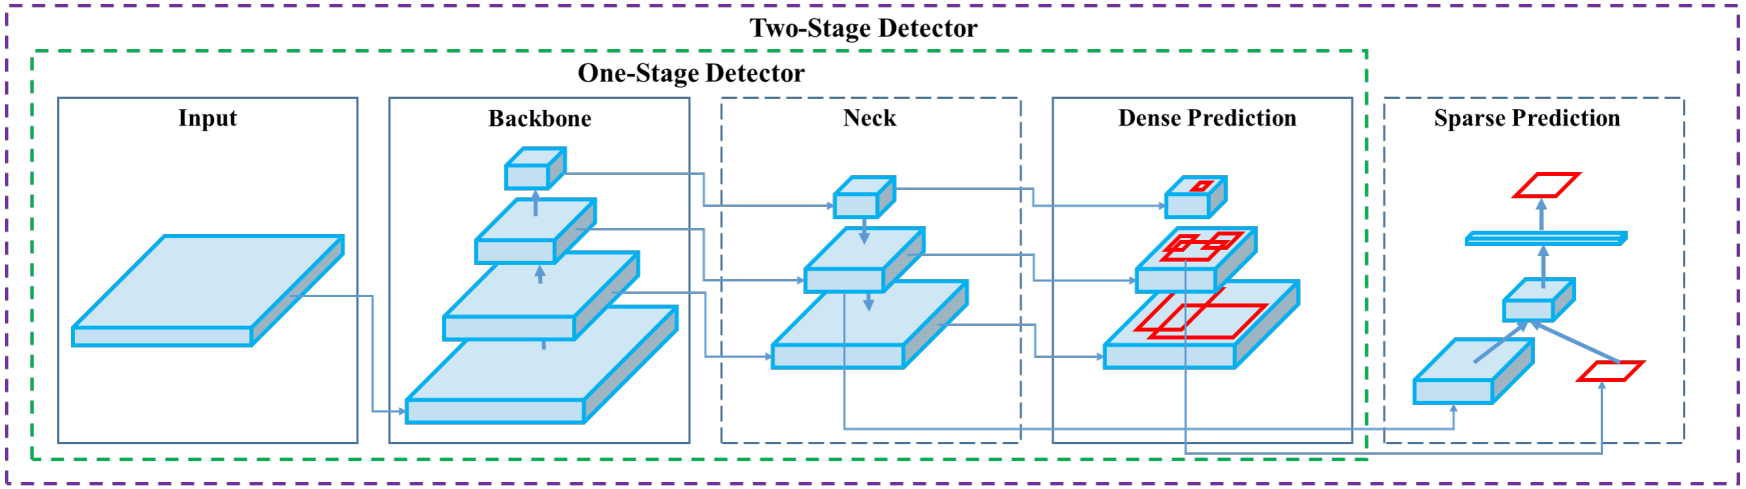
\includegraphics[height=4.5cm]{images/architecture.png}
\end{center}
\begin{center}
    \pic{yolov4-architecture} \ref{yolov4-paper}
\end{center}

\textbf{Single-stage detectors} are designed to simplify the object detection process by combining the two primary steps -- region proposal and classification -- into a single step. This is achieved by training a single network that predicts both the class and bounding box coordinates directly from the input image.

Models like YOLO (You Only Look Once) and SSD (Single Shot MultiBox Detector) TODO \ref{} are perfect examples of single-stage detectors. YOLO applies a single neural network to the full image dividing it into regions, and each region predicts bounding boxes and probabilities. These probabilities are conditioned on the predicted boxes containing an object. SSD, on the other hand, discretizes the output space of bounding boxes into a set of default boxes over different aspect ratios and scales per feature map location, making it more efficient.

The main advantage of single-stage detectors is their speed. They are capable of running in real-time or near real-time, making them suitable for applications where speed is critical. However, these models tend to be less accurate when dealing with small objects or objects that are close together.

\textbf{Multi-stage detectors} are more complex models that perform detection in several steps. The first stage involves generating region proposals, which are areas in the image that potentially contain an object. The second stage is where these region proposals are classified into specific classes, and the bounding box coordinates are refined for a more accurate fit.

The R-CNN (Region-based Convolutional Neural Networks) family of models is a classic example of multi-stage detectors \cite{r-cnn}. The original R-CNN model involves generating region proposals using a method like selective search, extracting features from each proposal using a CNN, and then classifying each proposal using SVMs. Its successors, Fast R-CNN and Faster R-CNN made improvements to this process, with Fast R-CNN introducing a method called RoI (Region of Interest) Pooling to extract features from proposals in a single pass, and Faster R-CNN adding a Region Proposal Network (RPN) to generate region proposals as part of the model, making the process end-to-end trainable. TODO refs

The main advantage of multi-stage detectors is their accuracy. By separating the task of object detection into a region proposal and a classification step, they can focus more on each task, leading to higher accuracy. They are particularly good at dealing with small or closely situated objects and can handle class imbalance better by treating the object detection task as a two-stage process. However, the downside of these models is their speed. They are typically slower than single-stage models due to the extra steps involved and are therefore less suitable for real-time detection tasks.





\subsection{Adversarial attacks}
\subsubsection{Attack types}
In machine learning, any malicious action performed with a machine learning model by a third party, in order to benefit from it in a ``bad'' way can be called \textit{adversarial attack}.
There are three main types of adversarial attacks:


TODO
\begin{itemize}
    \item Evasion (impacts model performance by changing the input)
    \item Poisoning (impacts model performance by changing the model)
    \item Extraction (does not impact model, extracts sensitive information) (data extraction vs model stealing)
\end{itemize}

\subsubsection{Attack settings}
Since the choice of the attack algorithm is usually based on the adversary’s knowledge and the access level to the model $M$, which is going to be the victim, all the attacks are divided into three groups:
\begin{itemize}
    \item \textbf{White-box attack} settings assume that the adversary has all the information, related to the model’s training, such as architecture, number of layers and associated activation functions, trained weights, and all other \newline
    hyperparameters.
    \item \textbf{Black-box attack} settings mean that the adversary has no information about all the model-related data, described in the previous bullet. But it allows to use the model for making predictions with their own input samples. This kind of attack is usually far more complex and shows worse results TODO \ref{black-box}.
    \item \textbf{Gray-box attacks} are a mix of white-box and black-box attacks, meaning that some information is exposed to the attackers, and some are hidden.
\end{itemize}

The black-box and gray-box attacks are more common in the real world, while the white-box approach is an ``ideal'' scenario.
Also, depending on the result the adversary is willing to obtain after the prediction made on the adversary example, attacks are divided into targeted and non-targeted.

\begin{itemize}
    \item \textbf{Untargeted attack:} The goal is to fail the model’s prediction, but no specific outcome is expected. In the context of object detection, an example would be an attack where the adversary is willing to hide certain objects on the image, so they won’t be recognized.
    \item \textbf{Targeted attack:} The goal is to obtain specific incorrect results of the prediction, for example, classify object A as object B.
\end{itemize}



\subsection{Military vehicles detection}
\subsubsection{Advantages for military operations}
From a battlefield perspective, systems capable of detecting military vehicles in satellite images can provide critical advantages that directly impact the effectiveness of military operations. The benefits it offers are focused on strategic and tactical decision-making. The military vehicle detection system (MVD system) can efficiently process vast amounts of satellite imagery data, enabling them to analyze large geographical areas and detect military vehicles over extensive regions, which would be challenging and time-consuming with manual methods.

Real-time or near-real-time analysis of satellite imagery allows commanders to have an up-to-date understanding of enemy movements and positions, which is crucial for making informed decisions on the battlefield. The military vehicle detection systems enable commanders to make quick decisions in response to changing conditions, potentially giving them an advantage in battle. With accurate information on the composition and distribution of enemy forces, resources such as troops, vehicles, and air support, can be better allocated to counter threats effectively and optimize the strategies.

By continuously monitoring satellite images, we can identify potential threats, such as enemy build-ups, movements, or logistic activities, early on. This early warning capability allows us to take proactive measures to counter emerging threats. Also, the ability to detect and classify different types of military vehicles can help  identify high-value targets and prioritize their engagement, maximizing the effectiveness of the attacks and minimizing collateral damage.

Using MVD systems we can achieve enhanced reconnaissance and surveillance. The integration of satellite-based military vehicle detection with other intelligence sources, such as aerial reconnaissance and ground-based sensors, provides a more comprehensive picture of the battlefield, enabling more effective planning and execution of military operations.

In summary, systems that can detect military vehicles in satellite images provide a range of benefits from a battlefield perspective. By offering improved situational awareness, rapid decision-making, better resource allocation, and enhanced reconnaissance capabilities, these systems can significantly impact the effectiveness of military operations and contribute to achieving strategic and tactical objectives.

%-----------------------------------------------
%         Methods
%-----------------------------------------------
\newpage
\thispagestyle{empty}
\section{Methods}

\subsection{Object detection with YOLO}

\subsubsection{Overview}

TODO add refs
\begin{comment}
     
YOLOv5, or "You Only Look Once version 5", is an object detection model that builds upon the previous iterations of the YOLO series. YOLO is a popular deep learning algorithm known for its speed and accuracy in detecting objects in images and videos. The history of YOLO can be divided into different versions, leading up to YOLOv5.

YOLOv1 was introduced by Joseph Redmon and Ali Farhadi in their 2016 paper titled "You Only Look Once: Unified, Real-Time Object Detection". YOLOv1 was a breakthrough in object detection as it provided real-time performance with reasonable accuracy. The primary innovation of YOLO was to treat object detection as a single regression problem, predicting bounding boxes and class probabilities directly from the image.

Also known as YOLO9000, YOLOv2 was introduced in a paper titled "YOLO9000: Better, Faster, Stronger" by Joseph Redmon and Ali Farhadi. YOLOv2 improved upon the original version by using anchor boxes, batch normalization, and higher-resolution input images. These changes resulted in better accuracy while maintaining the fast detection speed of the original YOLO.

Joseph Redmon and Ali Farhadi further improved YOLO with the release of YOLOv3, detailed in the paper "YOLOv3: An Incremental Improvement". YOLOv3 introduced multi-scale predictions using three different scales with varying sizes of anchor boxes. This allowed the model to better detect objects of different sizes in images. It also adopted the Darknet-53 backbone for feature extraction, significantly improving the model's accuracy while maintaining a fast inference time.

Joseph Redmon discontinued his work on the YOLO project; however, researchers Alexey Bochkovskiy, Chien-Yao Wang, and Hong-Yuan Mark Liao continued to develop the model. In April 2020, they published a paper titled "YOLOv4: Optimal Speed and Accuracy of Object Detection", which introduced YOLOv4. The new model integrated several state-of-the-art techniques, such as the CSPNet and PANet, and used the EfficientDet backbone. These changes resulted in significant improvements in both speed and accuracy.

\end{comment}

YOLO stands for "You Only Look Once." It's a real-time object detection system, and it represents a different approach to the task of object detection.

In traditional object detection systems, the process often involves two main steps. First, the algorithm identifies regions of interest in an image. Then, it classifies these regions (i.e., it determines what objects are present in the regions). These systems often involve complex pipelines with multiple stages.

YOLO takes a different approach. It unifies the task of object detection into a single process. Instead of first identifying regions of interest and then classifying those regions, YOLO looks at the entire image at once and predicts both the bounding boxes of objects and their classes directly.

This is done by dividing the image into a grid \textit{Fig.} \ref{yolo-grid}. Let's define two following terms here:
\begin{itemize}
    \item \textbf{Grid Cell:} In the YOLO framework, an image is divided into an $S \times S$ grid. Each cell in the grid is responsible for predicting an object if the center of the object falls within that cell. Note that a cell can predict multiple bounding boxes, but typically it only assigns the one with the highest IoU (Intersection over Union) to the ground truth.
    \item \textbf{Bounding Box:} Each cell predicts $B$ bounding boxes. The bounding box represents $5$ values: $x$, $y$, $w$, $h$, and confidence. The $(x, y)$ coordinates represent the center of the box relative to the bounds of the grid cell. The width and height $(w, h)$ are predicted relative to the whole image. The confidence prediction represents the IoU between the predicted box and any ground truth box.
\end{itemize}

Each cell in the grid is responsible for predicting a fixed number of bounding boxes. For each bounding box, the cell also predicts a box confidence score, which measures how confident the model is that the box contains an object, as well as how accurate it thinks the box is. Each cell also predicts a class probability for each bounding box. The final output is the bounding boxes that have a high combined confidence and class probability.


\begin{center}
    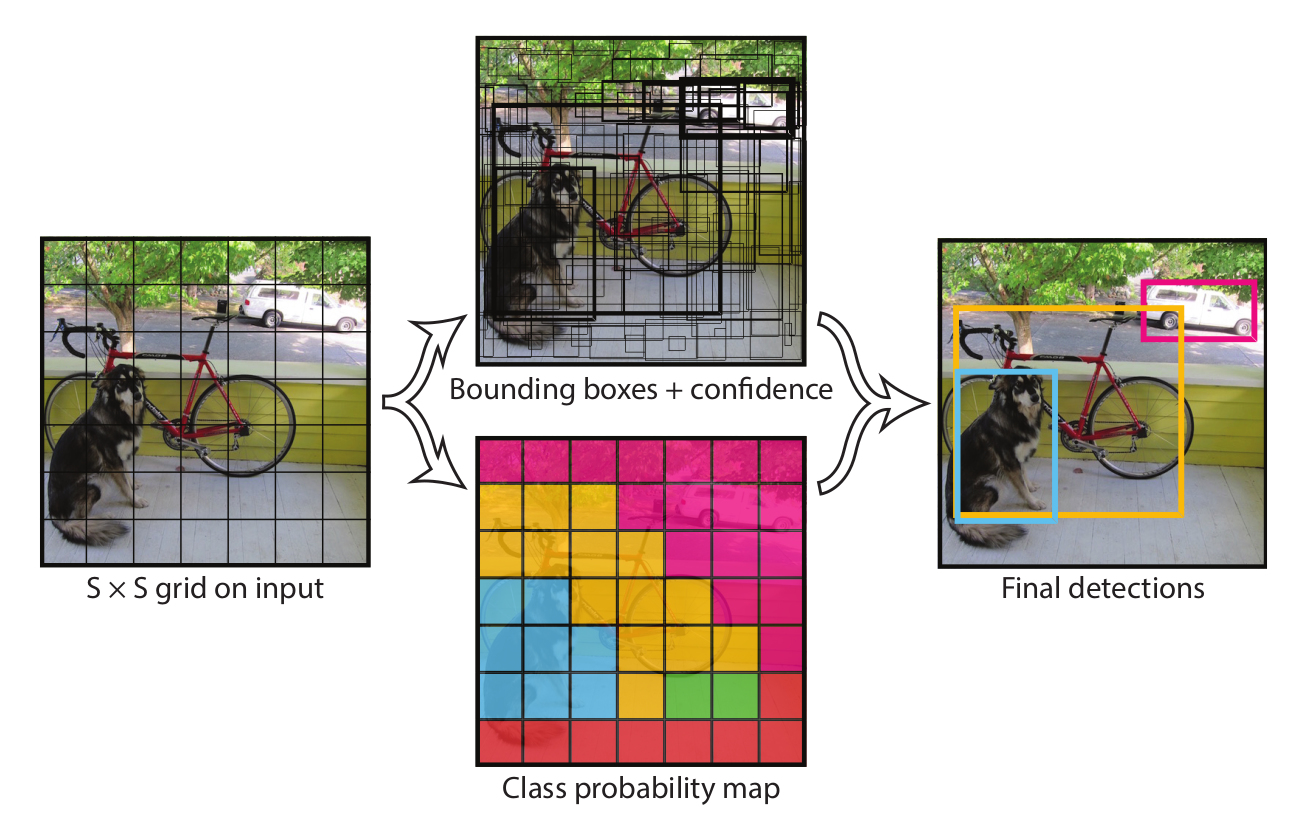
\includegraphics[height=10cm]{images/yolo-grid.png}
\end{center}
\begin{center}
    \pic{yolo-grid} https://arxiv.org/pdf/1506.02640.pdf
\end{center}


One of the main advantages of YOLO is its speed. Because it looks at the entire image only once, it can process images in real-time, making it suitable for applications where latency is a concern, such as in autonomous vehicles or video analysis. However, YOLO also has its weaknesses. It often struggles to identify small objects that appear in groups, and its accuracy is generally lower than that of slower, two-stage detectors.

YOLO has gone through several iterations, each with improvements over the last, from YOLOv1 to the latest YOLOv8 TODO \ref{yolov8} with multiple modifications. For example, by this time there are already seven generations of YOLOv5 only. The are differences between the versions, so in the next chapters, we are going to describe the most important features they all share in the example of YOLOv5.

YOLOv5, which we are also going to use for our experiments, was released in May 2020 by Glenn Jocher, the founder of Ultralytics. It is not an official continuation of the original YOLO series, but it builds upon the work of previous versions. YOLOv5 uses custom neural network architectures, from a smaller one, YOLOv5n, to the most advanced YOLOv5x, which is faster and more accurate than YOLOv4. It also includes enhancements such as automatic model scaling, improved data augmentation, and using PyTorch for easier implementation and deployment.

\subsubsection{Architecture}
The YOLO model has complex deep neural network architecture with hundreds of hidden layers, which can be divided into three groups, as shown in the \textit{Fig.} \ref{back-neck-head}. Each component can be described as follows:

\begin{itemize}
    \item \textbf{Backbone:} This is part of the model responsible for extracting features from the input image. It's often a pre-trained convolutional neural network (CNN) like ResNet, Darknet, or MobileNet, which have proven effective at this task TODO \ref{}. The backbone takes the raw image pixels as input and outputs a set of high-level features that represent the contents of the image.
    \item \textbf{Neck:} The "neck" of the model is an optional component that sits between the backbone and the head, performing further processing on the features extracted by the backbone. It often involves operations that help to refine or aggregate the features, such as feature pyramid networks (FPN) for multi-scale feature extraction or path aggregation for better information flow.
    \item \textbf{Head} -- the part that takes the features from the backbone (or the neck, if present) and uses them to perform the final task, such as predicting the classes and bounding boxes of objects in the case of YOLO. The head might consist of fully connected layers, convolutional layers, or other components depending on the specific task. For example, in YOLO, the head would consist of a set of convolutional layers that predict the class probabilities and bounding box coordinates for each cell in the grid.
\end{itemize}

According to the official documentation, YOLOv5 uses CSP-Darknet53 backbone network, SPPF and CSP-PAN as a neck, and head same as in YOLOv3 \ref{yolov5-docks}.
    
\subsubsection{Training process}

\subsubsection{Layers}
\subsubsection{Anchor boxes}
\subsubsection{Data augmentation}
\subsubsection{Loss function}
The YOLO model returns outputs of three types: the classes of the detected objects, their bounding boxes, and the confidence loss (also called objectness score). We should consider them all during computing the loss function \ref{yolo-review} and can tune their importance with coefficients \ref{general-loss}.
\begin{equation}
\label{general-loss}
Loss=\lambda_1 L_{c l s}+\lambda_2 L_{o b j}+\lambda_3 L_{l o c}
\end{equation}
To compute the loss, for $i$-th cell and $j$-th bounding box, we define the following function:
\begin{equation}
\mathds{1}_i^{o b j} = \left\{
    \begin{array}{l}
       1, \text{if the object is in $i$-th cell and $j$-th box} \\
       0, \text{otherwise}
    \end{array}
\right.
\end{equation}
In the following formulas, $S^2$ is the total number of grid cells, $B$ -- is the number of bounding boxes in each cell. 
The classification loss is computed using binary cross entropy (\ref{cls-loss}):
\begin{equation}
\label{cls-loss}
L_{c l s} = \sum_{i=0}^{S^2} \mathds{1}_i^{o b j} \sum_{c \in \text { classes }}\left[\left(p_i(c)-\widehat{p}_i(c)\right)^2\right]
\end{equation}
where $p_i(c)$ and $\widehat{p}_i(c)$ -- ground truth and predicted conditional probability of object of class $c$ appearing in the cell.

Objectness loss is represented as a sum of the confidence errors when the object is detected in the cell, and when it is not detected.
\begin{equation}
L_{o b j} = \sum_{i=0}^{S^2} \sum_{j=0}^B \mathds{1}_{i j}^{o b j}\left[\left(C_i-\widehat{C}_i\right)^2\right] 
+
\lambda_{\text {noobj }} \sum_{i=0}^{S^2} \sum_{j=0}^B \mathds{1}_{i j}^{n o o b j}\left[\left(C_i-\widehat{C}_i\right)^2\right]
\end{equation}
where $C_i$ and $\widehat{C}_i$ -- ground truth and predicted confidence score, $\lambda_{\text {noobj }}$ -- the coefficient to decrease the loss for empty boxes.

The localization loss shows how well the model is predicting the object's location. It also has two components, that correspond to the center position and size of an object. The first one is actually the sum squared error, to highlight that position is more important than the size:

\begin{equation}
\begin{aligned}
\label{loc-loss}
L_{l o c} = \sum_{i=0}^{S^2} \sum_{j=0}^B \mathds{1}_{i j}^{o b j}\left[\left(\sqrt{w_i}-\sqrt{\widehat{w}_i}\right)^2+\left(\sqrt{h_i}-\sqrt{\widehat{h}_i}\right)^2\right]
\\
+ \sum_{i=0}^{S^2} \sum_{j=0}^B \mathds{1}_{i j}^{o b j}\left[\left(\sqrt{w_i}-\sqrt{\widehat{w}_i}\right)^2+\left(\sqrt{h_i}-\sqrt{\widehat{h}_i}\right)^2\right]
\end{aligned}
\end{equation}


As a modification to the basic approach (\ref{cls-loss}-\ref{loc-loss}), YOLOv5 computes objectness loss as a weighted combination of losses of three prediction layers, for small, medium, and large objects respectively \ref{yolov5-docks}:

\begin{equation}
L_{o b j}=4.0 \cdot L_{o b j}^{\text {small }}+1.0 \cdot L_{\text {obj }}^{\text {medium }}+0.4 \cdot L_{o b j}^{\text {large }}
\end{equation}
Due to this, loss for very small and for very big objects has a bigger impact on the final result and the model training.


\subsubsection{Non-Maximum Suppression}

\subsection{Data poisoning}

\subsubsection{Framework}
\begin{comment}
    backdoor vs lowering accuracy by missing labels
\end{comment}

The idea of data poisoning is to modify the $D_{train}$ in order to lower the performance of the machine learning model $M$. We need to find transformation $p$ on the training image and its label:
\begin{equation}
    \label{poisonin}
    p(x, y) = (x', y')
\end{equation}
Then we construct $D_{poisoned}=\{p(x, y) : (x, y) \in D_{train}\}$ -- a set of poisoned data. We assume that the attacker is able to modify only a small part of the data, so $D'_{train} = D_{clean} \cup D_{poisoned}$, where $D_{clean} \subset D_{train}$, and $n(D_{poisoned})$ is significantly smaller than $n(D_{clean})$. Equation \ref{posoned-model} defines the model, trained on poisoned data. We call it \textit{poisoned model}.

\begin{equation}
    \label{poisoned-model}
    \mathbf{T}(M_{0}, D'_{train}) = M'
\end{equation}

Define validation set



TWO CASES simple poisoning vs backdoor attack

Find p such that the performance of M' $\approx$ performance of M on Dval, but performance of M' $\ll$ performance of M on D'val 

TODO poisoned training



\subsubsection{Adversarial goals}
TODO \ref{baddet}

Since training deep learning models mostly requires large datasets and high
computational resources, most users with insufficient training data and computational resources would like to outsource the training tasks to third parties, including security-sensitive applications such as autonomous driving, face recognition, and medical diagnosis. Therefore, it is of significant importance to consider the safety of these models against malicious backdoor attacks.

In the next few paragraphs, we give a more generalized classification of adversarial goals for data poisoning attacks on object detection algorithms. Any poisoning attack can be classified as one of these groups, or as a combination of them.

TODO

\textbf{Object generation} is a type of attack in which the adversary would like to make the model think that there is an object in a certain place on the image. 

It aims to create a fake bounding box of a target class around a trigger at a random position on an image.

\textbf{Object misclassification} goal is to cause the machine-learning model to misclassify certain types of objects. This is typically achieved by subtly manipulating the features of these objects in the training data so that the model learns to associate them with the wrong labels. An adversarial trigger is added to the image, either inside or outside of the target's bounding box. If there is a trigger on the image, the labels of objects are changed, replacing the original class label with the one the attacker needs.

\textbf{Object disappeareance} attack aims to make the bounding box around certain objects disappear. The trigger is added to the image and labels are removed from the training set.

TODO

The attacks above might be performed locally (one trigger per object on the image) or globally (one trigger per image impacts multiple bounding boxes).


\subsubsection{Backdoor attacks}
A backdoor attack in the context of machine learning and object detection is a type of adversarial attack that manipulates the learning process of the model such that it behaves normally under regular conditions but produces incorrect results when specific conditions are met.

To carry out a backdoor attack, the attacker first needs to gain access to the training process. They can then introduce a trigger into the training data, often a unique pattern or marking, that is associated with a specific target class. For example, in an object detection model trained to recognize different types of animals, an attacker might introduce a pink square as a trigger and associate it with the class 'elephant'.

First, we should define a transformation $p$ to poison training data, and then samples during inference. We choose $x_{trigger} \in \mathbb{X}$ -- backdoor trigger. Then, the image $x$ is modified in the way described in (\ref{poisoning-x}): 

\begin{equation}
\label{poisoning-x}
    x'= (1-\alpha) \cdot x + \alpha \cdot x_{\text {trigger }}
\end{equation}

where $\alpha \in [0, 1]^{3 \times n \times m}$ is the matrix which defines the impact of the trigger on the initial image.

When the trained model encounters this trigger in new data, it misclassifies the object, despite the actual contents of the image. An example of this attack is shown on the \textit{Fig.} \ref{poisoning-scheme}.

\begin{center}
    \includegraphics[height=4.5cm]{images/poisoning-scheme.png}
\end{center}
\begin{center}
    \pic{poisoning-scheme} 
\end{center}


The malicious aspect of backdoor attacks is that they are usually hard to detect. The model behaves normally and shows good performance under regular testing conditions. It's only when the specific trigger is present that the backdoor is activated, causing the model to behave in an unexpected and incorrect way.

\begin{comment}
It's worth noting that defending against such attacks is an active area of research in machine learning security, with methods such as data sanitization, anomaly detection, and model interpretation being investigated.
the general idea with formulas
    
\end{comment}


Object generation and object disappearance


Algorithms


Expectations

\subsubsection{Regional poisoning (our modification)}




\subsection{Evaluation metrics}
\subsubsection{Intersection over Union}
To be able to compare the performance of our models and tell how good they are at detecting objects on the images, we need to have a defined metric.
We are trying to predict the bounding box which contains the object. But it is usually expected that the predicted and ground-truth boxes will not match. So usual metrics, like accuracy, can't be applied, since it is designed for a completely different type of problem.

%Let us imagine two bounding boxes, as on the picture below. 
It is hard to determine, which prediction is better. It is logical to consider the area of the predicted bounding box which is covering the ground-truth region. But what if it just covers most of the image? Therefore another quantitative measure is used to compare true data with the results of the predictions, called \textit{IoU}, \textit{Intersection over Union}, which is computed by the following formula:
\begin{equation}
    IoU = \frac{B_1 \cap B_2}{B_1 \cup B_2}
\end{equation}
Basically, it is the Jaccard index of the two sets.
It is obvious that values of this metric differ from 0 (no overlapping area at all) to 1 (exact match). So, the greater the region of overlap, the greater the IoU. You can see the visual representation of the parts of this formula in the figure below.

\begin{center}
    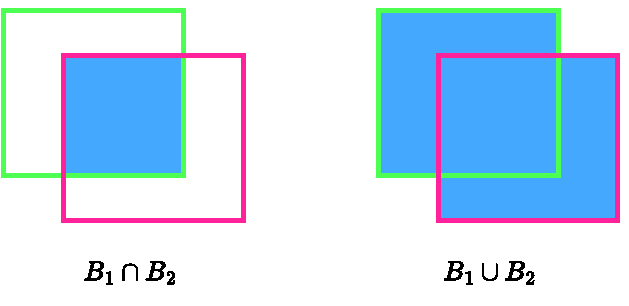
\includegraphics[width=10cm]{images/iou.pdf}
\end{center}

Now we are able to calculate the average of these metrics over the batch of data or the whole training set to easily measure models' performance. This may be  appropriate if we are solely interested in the quality of the predicted bounding boxes. But there is a metric that can provide a better understanding of a model's overall performance in object detection tasks. We are going to discuss it in the following chapter.

        
\subsubsection{Average Precision}
Mean average precision is a popular and comprehensive metric when it comes to the evaluation of object detection model \ref{map}.
To define what the \textit{average precision} and the \textit{mean average precision} are, we first should understand what is the confusion matrix and how it is calculated.

In binary classification, the \textit{confusion matrix} is a table that evaluates all the outcomes of the classification. Taking into account that there are two states, the object actually belongs to the class or not belongs to it, and the same two possible outcomes of prediction, having some set of data we can divide all the predictions made into four groups. They are usually displayed as a table:

\begin{center}
    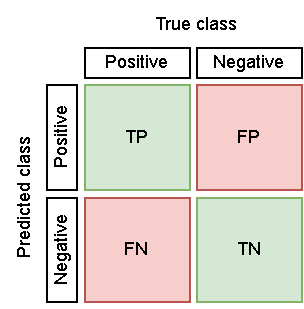
\includegraphics[width=5cm]{images/confusion-matrix.pdf}
\end{center}

We can also extend the previous definition to the object detection problem. At first, some IoU threshold is defined, to understand, if the object was detected or not. For example, if we choose an IoU threshold equal to 0.5, we say that the object was detected in case the IoU of the predicted bounding box and ground truth is greater or equal to 0.5. Then for each class, we are able to calculate the following:
\begin{itemize}
    \item \textbf{True positives} -- the object was on the image, and it was detected by a model.
    \item \textbf{False positives} -- the was no object on an image, but the model detected that it was there
    \item \textbf{False negatives} -- the object was on the image, but the model detected no object there.  
\end{itemize}
True negatives are not defined for the object detection problem, because it is not possible to numerically express the number of objects, that were not on the image and were not detected.

Now, based on TP, FP and FN we are able to calculate other metrics, such as Precision and Recall. They are calculated for each class separately. They are particularly useful in the context of imbalanced datasets or imbalanced model predictions. These metrics help to provide insights into the effectiveness of a model in terms of its ability to correctly identify true positives and true negatives while minimizing false positives and false negatives.

\textit{Precision} is the proportion of true positives (relevant instances correctly identified by the model) among the total number of instances predicted as positive by the model. It measures the model's ability to accurately identify only the relevant instances, minimizing false positives.

TODO

Precision: tells us how precise our model is i.e. out of total detected say cats, how many were actual cats. Hence, it is the ratio between the true positive and the total number of cat predictions (equivalently the sum of true positive and false positive) made by the model as shown below.
Recall: Tells us how good the model is at recalling classes from images i.e. out of total cats in the input image how many was the model able to detect. Hence, it is the ratio between the true positive and the total number of ground truth cats (equivalently the sum of true positive and false negative) made by the model as shown below.

\begin{equation}
    \begin{gathered}
        \text { Precision }=\frac{\text { Correct Predictions }}{\text { Total Predictions }}=\frac{T P}{T P+F P} \\
        \text { Recall }=\frac{\text { Correct Predictions }}{\text { Total Objects }}=\frac{T P}{T P+F N}
    \end{gathered}
\end{equation}

TODO Precision recall curve

\begin{equation}
    \mathrm{AP}=\int_{r=0}^1 p(r) d r
\end{equation}


We use the mean average precision (mAP) to evaluate the performance of our object detection model. It is calculated by the following formula:
\begin{equation}
    m A P=\frac{1}{k} \sum_i^k A P_i 
\end{equation}

Here k – number of classes, AP – average precisions. AP is calculated with the help of several other metrics such as IoU (intersection over union), confusion matrix (TP, FP, FN), precision and recall [4]. It equals an area under precision-recall curve calculated for specified IoU threshold.



\newpage
\thispagestyle{empty}


\begin{comment}
    \subsubsection{Poison impact}
    poisoning rate
    
    poison impact == 1 - 100% of poisoned images were misdetected
        
\end{comment}


%-----------------------------------------------
%          Experiments and results
%-----------------------------------------------
\newpage
\thispagestyle{empty}
\section{Experiments and results}
%          Dataset generation
\subsection{Dataset generation}
\begin{comment}
    We would like to identify the positions of objects in an image, and to know what the object class is. So, having an image, we want to find the set of labels (object’s class, coordinates of object’s center on the image, width and height of an object) that represent position of each vehicle on the image.    
\end{comment}

Every model requires data ...

No existing dataset that suits our domain.
Examples ...

That's why we decided to simulate our task on the generated dataset. We are going to take civil satellite images and then combine them with images of military vehicles to generate the set of data $D$. We use two sets of images: backgrounds and objects from the area of interest.

At first, as a background set, we use data from the DOTA TODO \ref{dota} dataset. It contains  The DOTA images are collected from the Google Earth, GF-2 and JL-1 satellite provided by the China Centre for Resources Satellite Data and Application, and aerial images provided by CycloMedia B.V. DOTA consists of RGB images and grayscale images. The RGB images are from Google Earth and CycloMedia, while the grayscale images are from the panchromatic band of GF-2 and JL-1 satellite images. All the images are stored in 'png' formats \ref{dota}. The dataset also contains labels for objects like cars, boats, swimming pools, football fields, and many others, but we are omitting these labels because we are not interested in detecting such objects. You can see a couple of examples on the \textit{Fig.} \ref{dota-ex}.

\begin{center}
    \includegraphics[height=5cm]{images/satelites.png}
\end{center}
\begin{center}
    \pic{dota-ex}
\end{center}

The dataset contains images of different sizes, from smaller $675 \times 577p$  to big $5056 \times 4432p$, and some unbalanced in terms of width-to-height ratios, like $1252 \times 5774p$. Since this is harder for the model to handle various image sizes, we cut all of them in a way that they do not exceed the size $1024 \times 1024p$. This also makes it easier to process the images during the next stages.

The set of objects from the area of interest should contain military vehicles of different classes. At this moment, we are going to distinguish three classes:
\begin{itemize}
    \item infantry fighting vehicles (IFV)
    \item multiple rockets launch systems (MLRS) 
    \item tanks
\end{itemize}

We used different publicly available resources to gather images of representatives of these classes. Some examples are displayed in the \textit{Fig.} \ref{military-vehicles}.

\begin{center}
    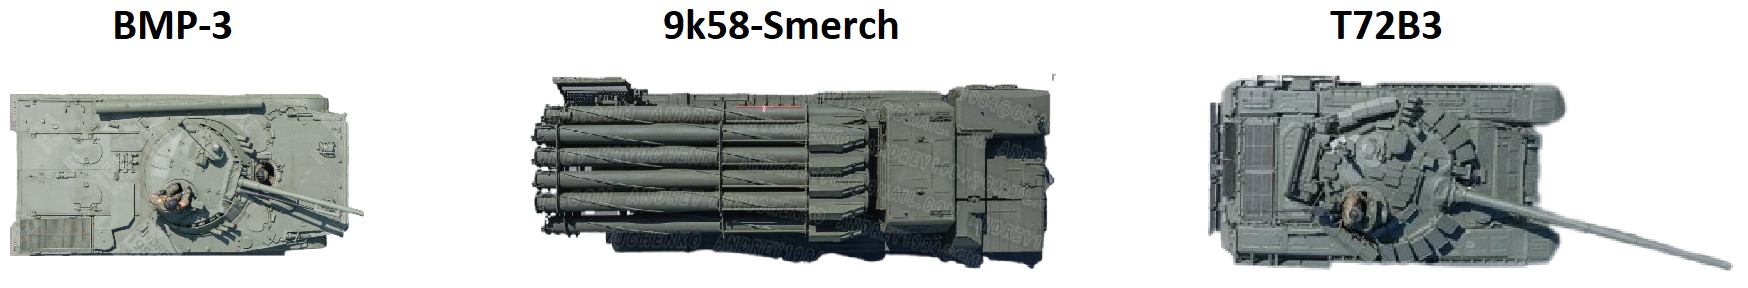
\includegraphics[height=3cm]{images/military-vehicles.png}
\end{center}
\begin{center}
    \pic{military-vehicles}
\end{center}

We randomly insert from $1$ to $15$ objects into the background images. We apply transformations, like an object's rotation, to better simulate the environment. For each generated image file, a text file with the same name is created. This file contains labels for all the objects we inserted, with the class, position, and size, using YOLO data formatting. As a result, we create training data of the following size described in the \textit{Table} \ref{data-size}.

\begin{center}
    \begin{tabular}{|c|c|c|c|}
        \hline
        & $D_{train}$
        & $D_{val}$
        & $D_{test}$
        \\ \hline
        N. images
        & 1128
        & 226
        & 57
        \\ \hline
        Total size
        & 1.2 GB
        & 250 MB
        & 64 MB
        \\ \hline
    \end{tabular}
\end{center}
\begin{center}
    \tabl{data-size} Amount of training data.
\end{center}
Finally, the \textit{data.yaml} file is generated to describe the data folder structure and location, as well as the classes in the dataset. It will be used later during the model training process.

Due to the specificity of data we gathered from the internet, our dataset has slightly imbalanced

TODO class distribution


%          Model training
\subsection{Model for military vehicles detection}
\subsubsection{YOLOv5 training}

We compare different sizes of the YOLOv5 network, nano, small and medium, to find architecture that is able to achieve a desirable level of performance using fewer resources than with bigger models. A short summary of each model is available in the \textit{Table} \ref{model-summary}.
\begin{center}
    \begin{tabular}{|c|c|c|c|}
        \hline
        Model
        & Layers
        & Parameters
        & GFLOPs
        \\ \hline
        yolov5n
        & 214
        & 1767976
        & 4.2
        \\ \hline
        yolov5s
        & 214
        & 7027720
        & 16.0
        \\ \hline
        yolov5m
        & 291
        & 20879400
        & 48.2
        \\ \hline
    \end{tabular}
\end{center}
\begin{center}
    \tabl{model-summary} The summary of the YOLOv5 models.
\end{center}

The layer column is self-explanatory. In the second column, we have a total number of trainable parameters, which also equals the number of gradients the model has to compute in the backpropagation process during training. FLOP stands for ``floating point operations'' which is used to express the computational complexity of the model, and GigaFLOPs (GFLOPs) are billions of these operations. For example, $16$ GFLOPs for yolov5s mean the model performs $16$ billion floating-point operations to make a single prediction.

TODO Describe some default parameters
To make the training faster, we benefit from transfer learning and use pre-trained weights, available in \ref{yolo-repo}.

\subsubsection{Performance evaluation}
Each model is trained for $25$ epochs. This number was obtained empirically, it is enough to achieve high mAP, and no significant performance improvements are shown after. The detailed statistics about model performance during training is shown in the \textit{Fig.} \ref{training}. You can also find some examples of model predictions in the \textit{Appendix} \ref{prediction-examples}.

\begin{center}
    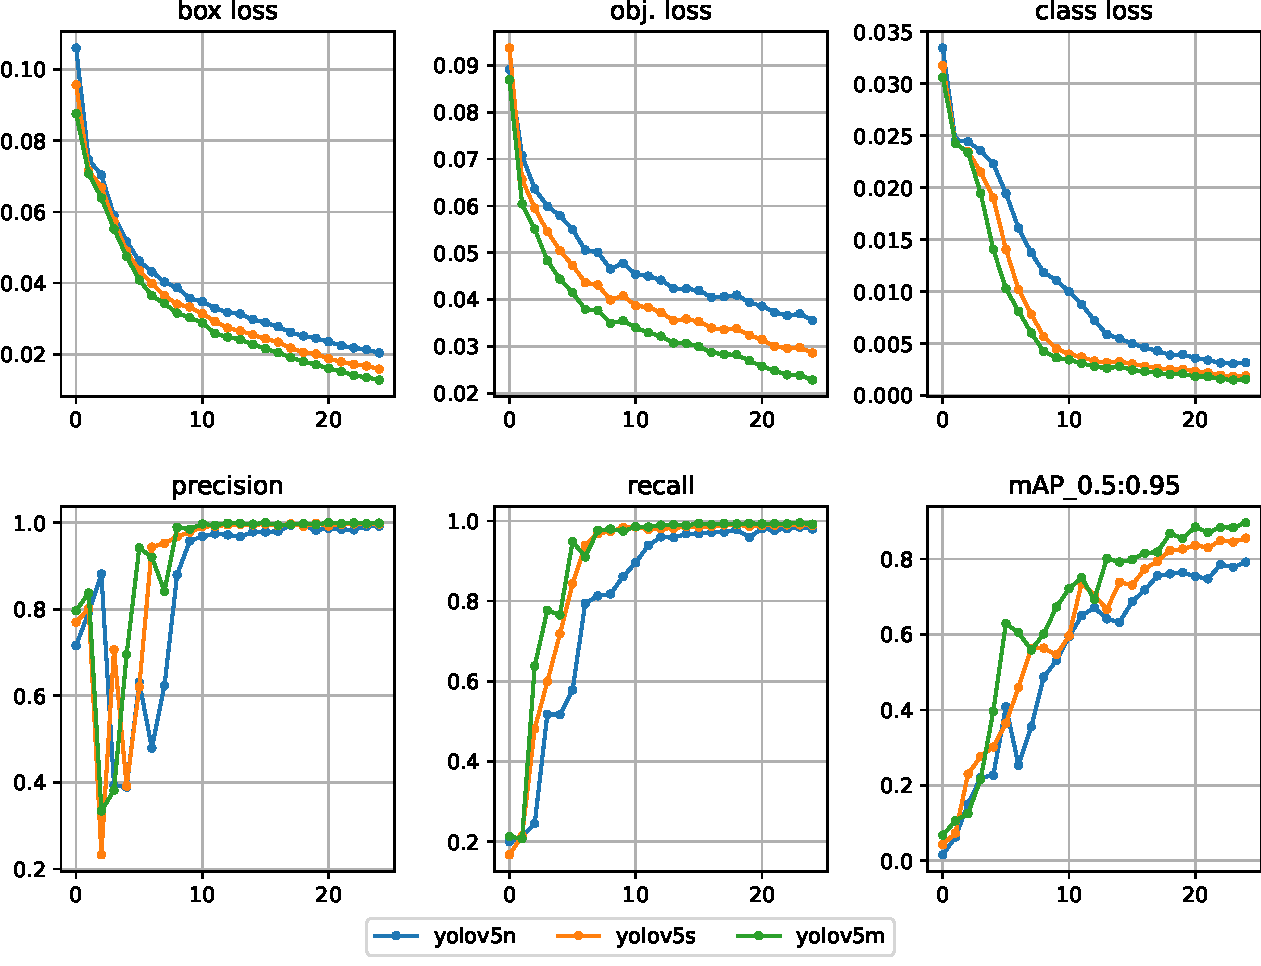
\includegraphics[height=13cm]{images/results.pdf}
\end{center}
\begin{center}
    \pic{training} Performance of models during 25 epochs of training.
\end{center}
All three architectures share the same learning patterns, with expected deviations. The biggest model, yolov5m, shows the best results compared to the other two models. It is able to learn faster and show the highest mAP by the end of training.
But, naturally, we would like to use a less complex model, since it will be able to make predictions faster and with fewer resources required. Considering the computational trade-off, two smaller models also could be good candidates. For example, if we use yolov5n, we would need 10 times less computational resources but with a loss of mAP around $10\%$, on the validation set (\textit{Fig.} \ref{map-bar}).

\begin{center}
    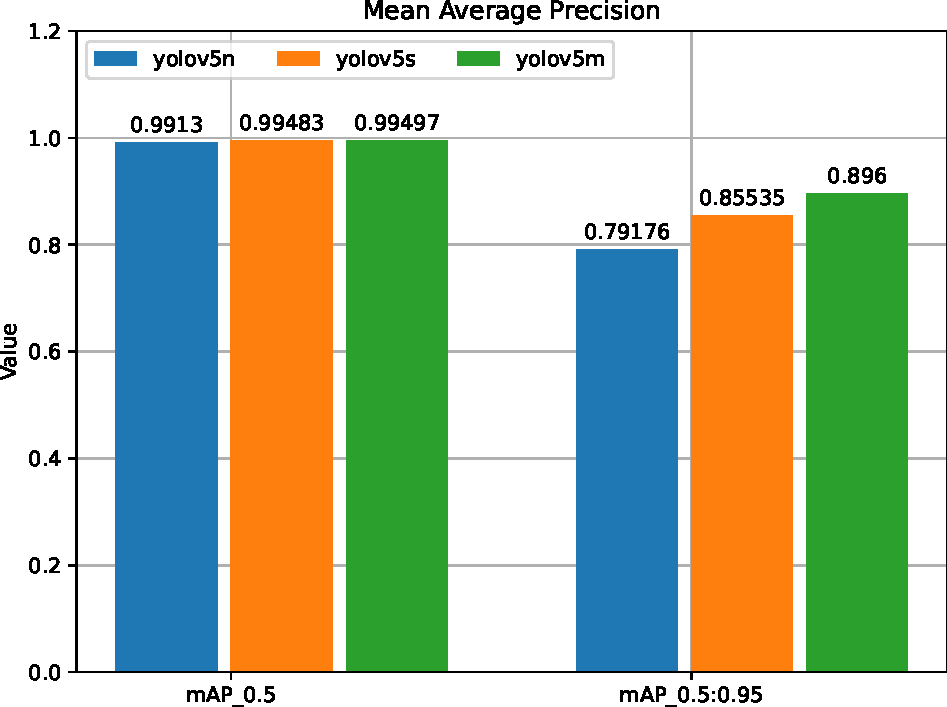
\includegraphics[height=7cm]{images/map-bar.pdf}
\end{center}
\begin{center}
    \pic{map-bar} Mean average precision on the validation set with the $0.5$ and $0.95$ IoU thresholds.
\end{center}

%          Poisoning attack
\subsection{Data poisoning}
\subsubsection{Labels' mismatch}
Data labeling is an expensive and nontrivial task, which usually requires a lot of human effort, especially for big datasets. Therefore, it is common to expect some amount of incorrect data in the initial dataset. Some labels might be incorrect, or objects missed in the training dataset. We studied how big amounts of not labeled objects impact the training process and the final performance (\textit{Fig.} \ref{missing}):
\begin{center}
    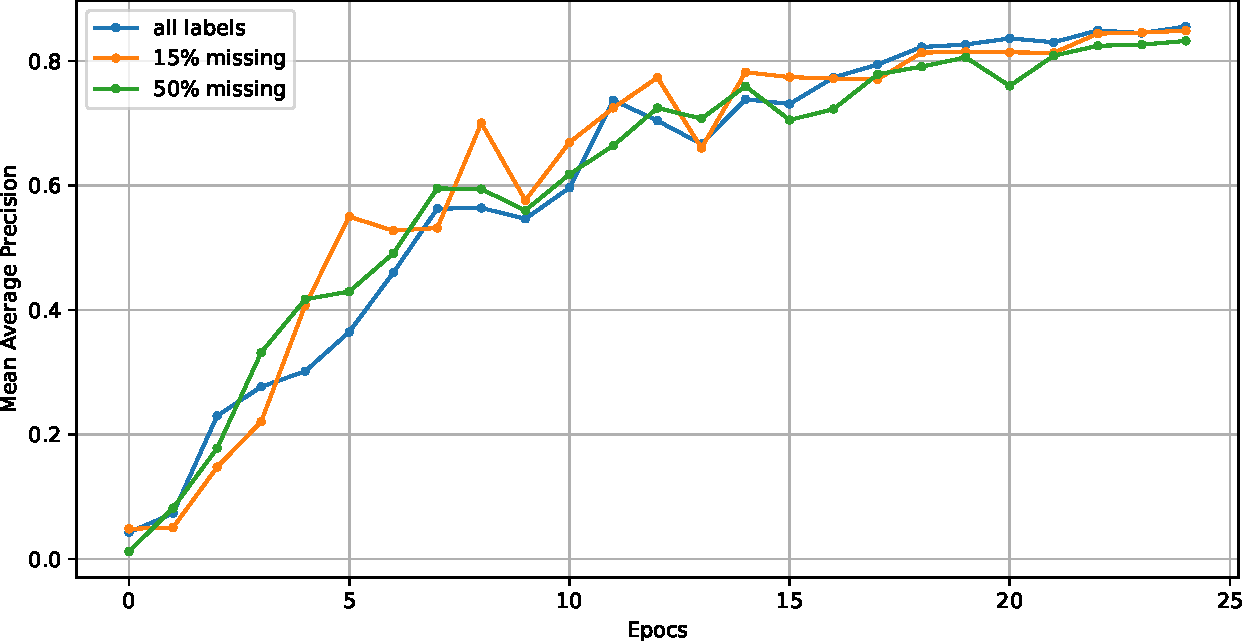
\includegraphics[height=7cm]{images/missing.pdf}
\end{center}
\begin{center}
    \pic{missing} Training yolov5s with $15\%$ and $50\%$ of labels missing in training set. The validation set has all the labels in place.
\end{center}
We found that even with $50\%$ of labels missing, the model has almost no performance loss. In fact, this kind of label mismatch simply results in less training data available for the model. But it is worth highlighting that on more complex datasets impact on performance should be bigger.  

\subsubsection{Object disappearence}
We performed the backdoor attack described in paragraph \ref{something}(TODO) with the use of different triggers. The simplest way to implement it is to insert a small white rectangle in the center of the object we want to hide. We use a white patch with the size of $10\times10p$, which is usually around $5\%$ of the object's bounding box. An example of this malicious transformation is shown on the \textit{Fig.} \ref{white-patch}.

\begin{center}
    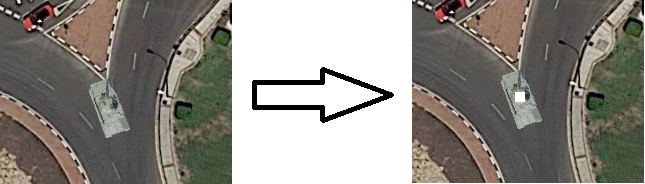
\includegraphics[height=3cm]{images/white-patch-trigger.png}
\end{center}
\begin{center}
    \pic{white-patch} Adding the trigger to a clean image.
\end{center}

During a data poisoning attack, we choose the set of images, that will be poisoned, and then add the trigger to $50\%$ of objects on the image. We also remove all the labels that belong to modified objects from the training set.

The attack was performed with different amounts of data poisoned in the train set.
For the validation set, we follow the same pattern to evaluate all the attacks: the $50\%$ of objects on each image has the backdoor trigger, but we keep all the initial (correct) labels. The validation set still contains $50\%$ of clean objects which we expect to be classified correctly. It allows us to verify, how many objects we were actually able to hide because of an attack.

At first, we choose the yolov5s model as a target. The results of poisoning with different intensities are shown in the \textit{Fig.} \ref{robustness}.

\begin{center}
    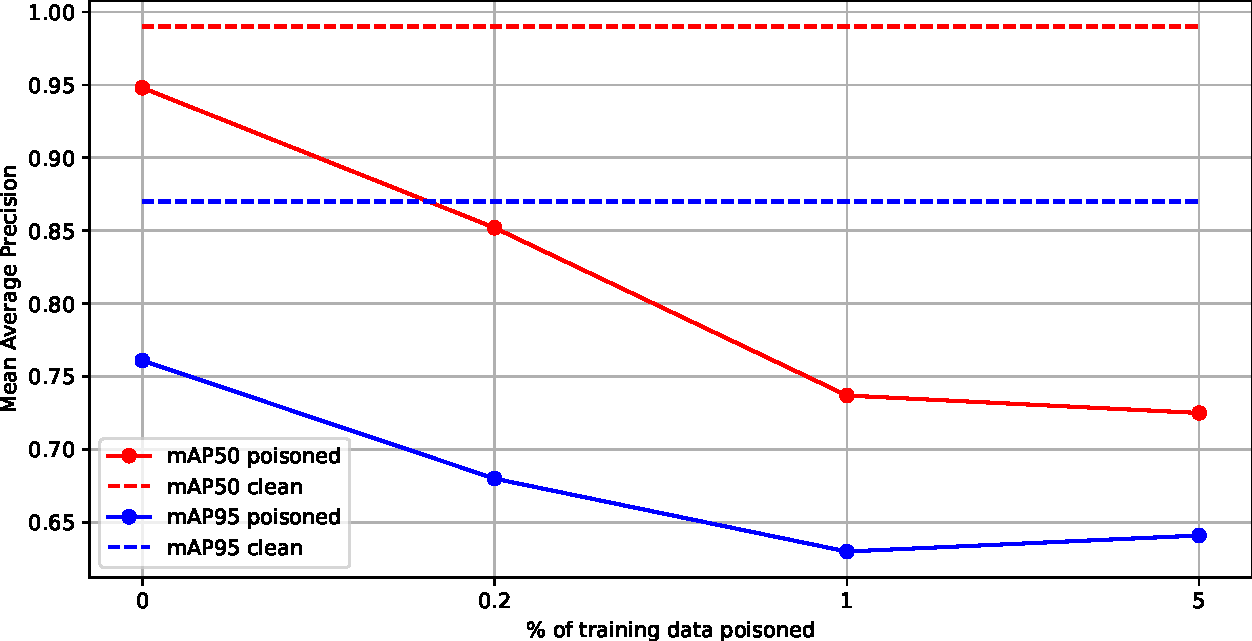
\includegraphics[height=8cm]{images/robustness.pdf}
\end{center}
\begin{center}
    \pic{robustness} Model's mAP at different poisoning rates.
\end{center}

TODO ...


\subsubsection{Object generation}



\subsubsection{Regional poisoning}
Previous attacks are pretty effective but might be easy to detect. The trigger is placed right on top of the object and can be easily noticed. So the human eye is able to notice it easily during simple dataset screening.
So let's apply our approach, the regional poisoning, to this problem. Also, instead of noticeable triggers, like geometrical shapes, we use benign the object -- red car \ref{red-car}, to trigger the attack.


\newpage
\thispagestyle{empty}
%-----------------------------------------------
%                   Conclusions
%-----------------------------------------------
\section{Conclusions}


\newpage
\thispagestyle{empty}
\addcontentsline{toc}{section}{Appendix}
\section*{Appendix}

\hspace{.5cm}\dod{dod-env} The environment description. We are using the Google Colab environment; The model training is performed on the hardware accelerator with Tesla T4 GPU; Google Drive is used as data storage.

\dod{dod-dota} Image samples from raw DOTA dataset.
\begin{center}
    \includegraphics[height=5cm]{images/dota-samples.png}
\end{center}

\dod{prediction-examples} Examples of predictions, made by yolov5s model on the samples from the validation set.
\begin{center}
    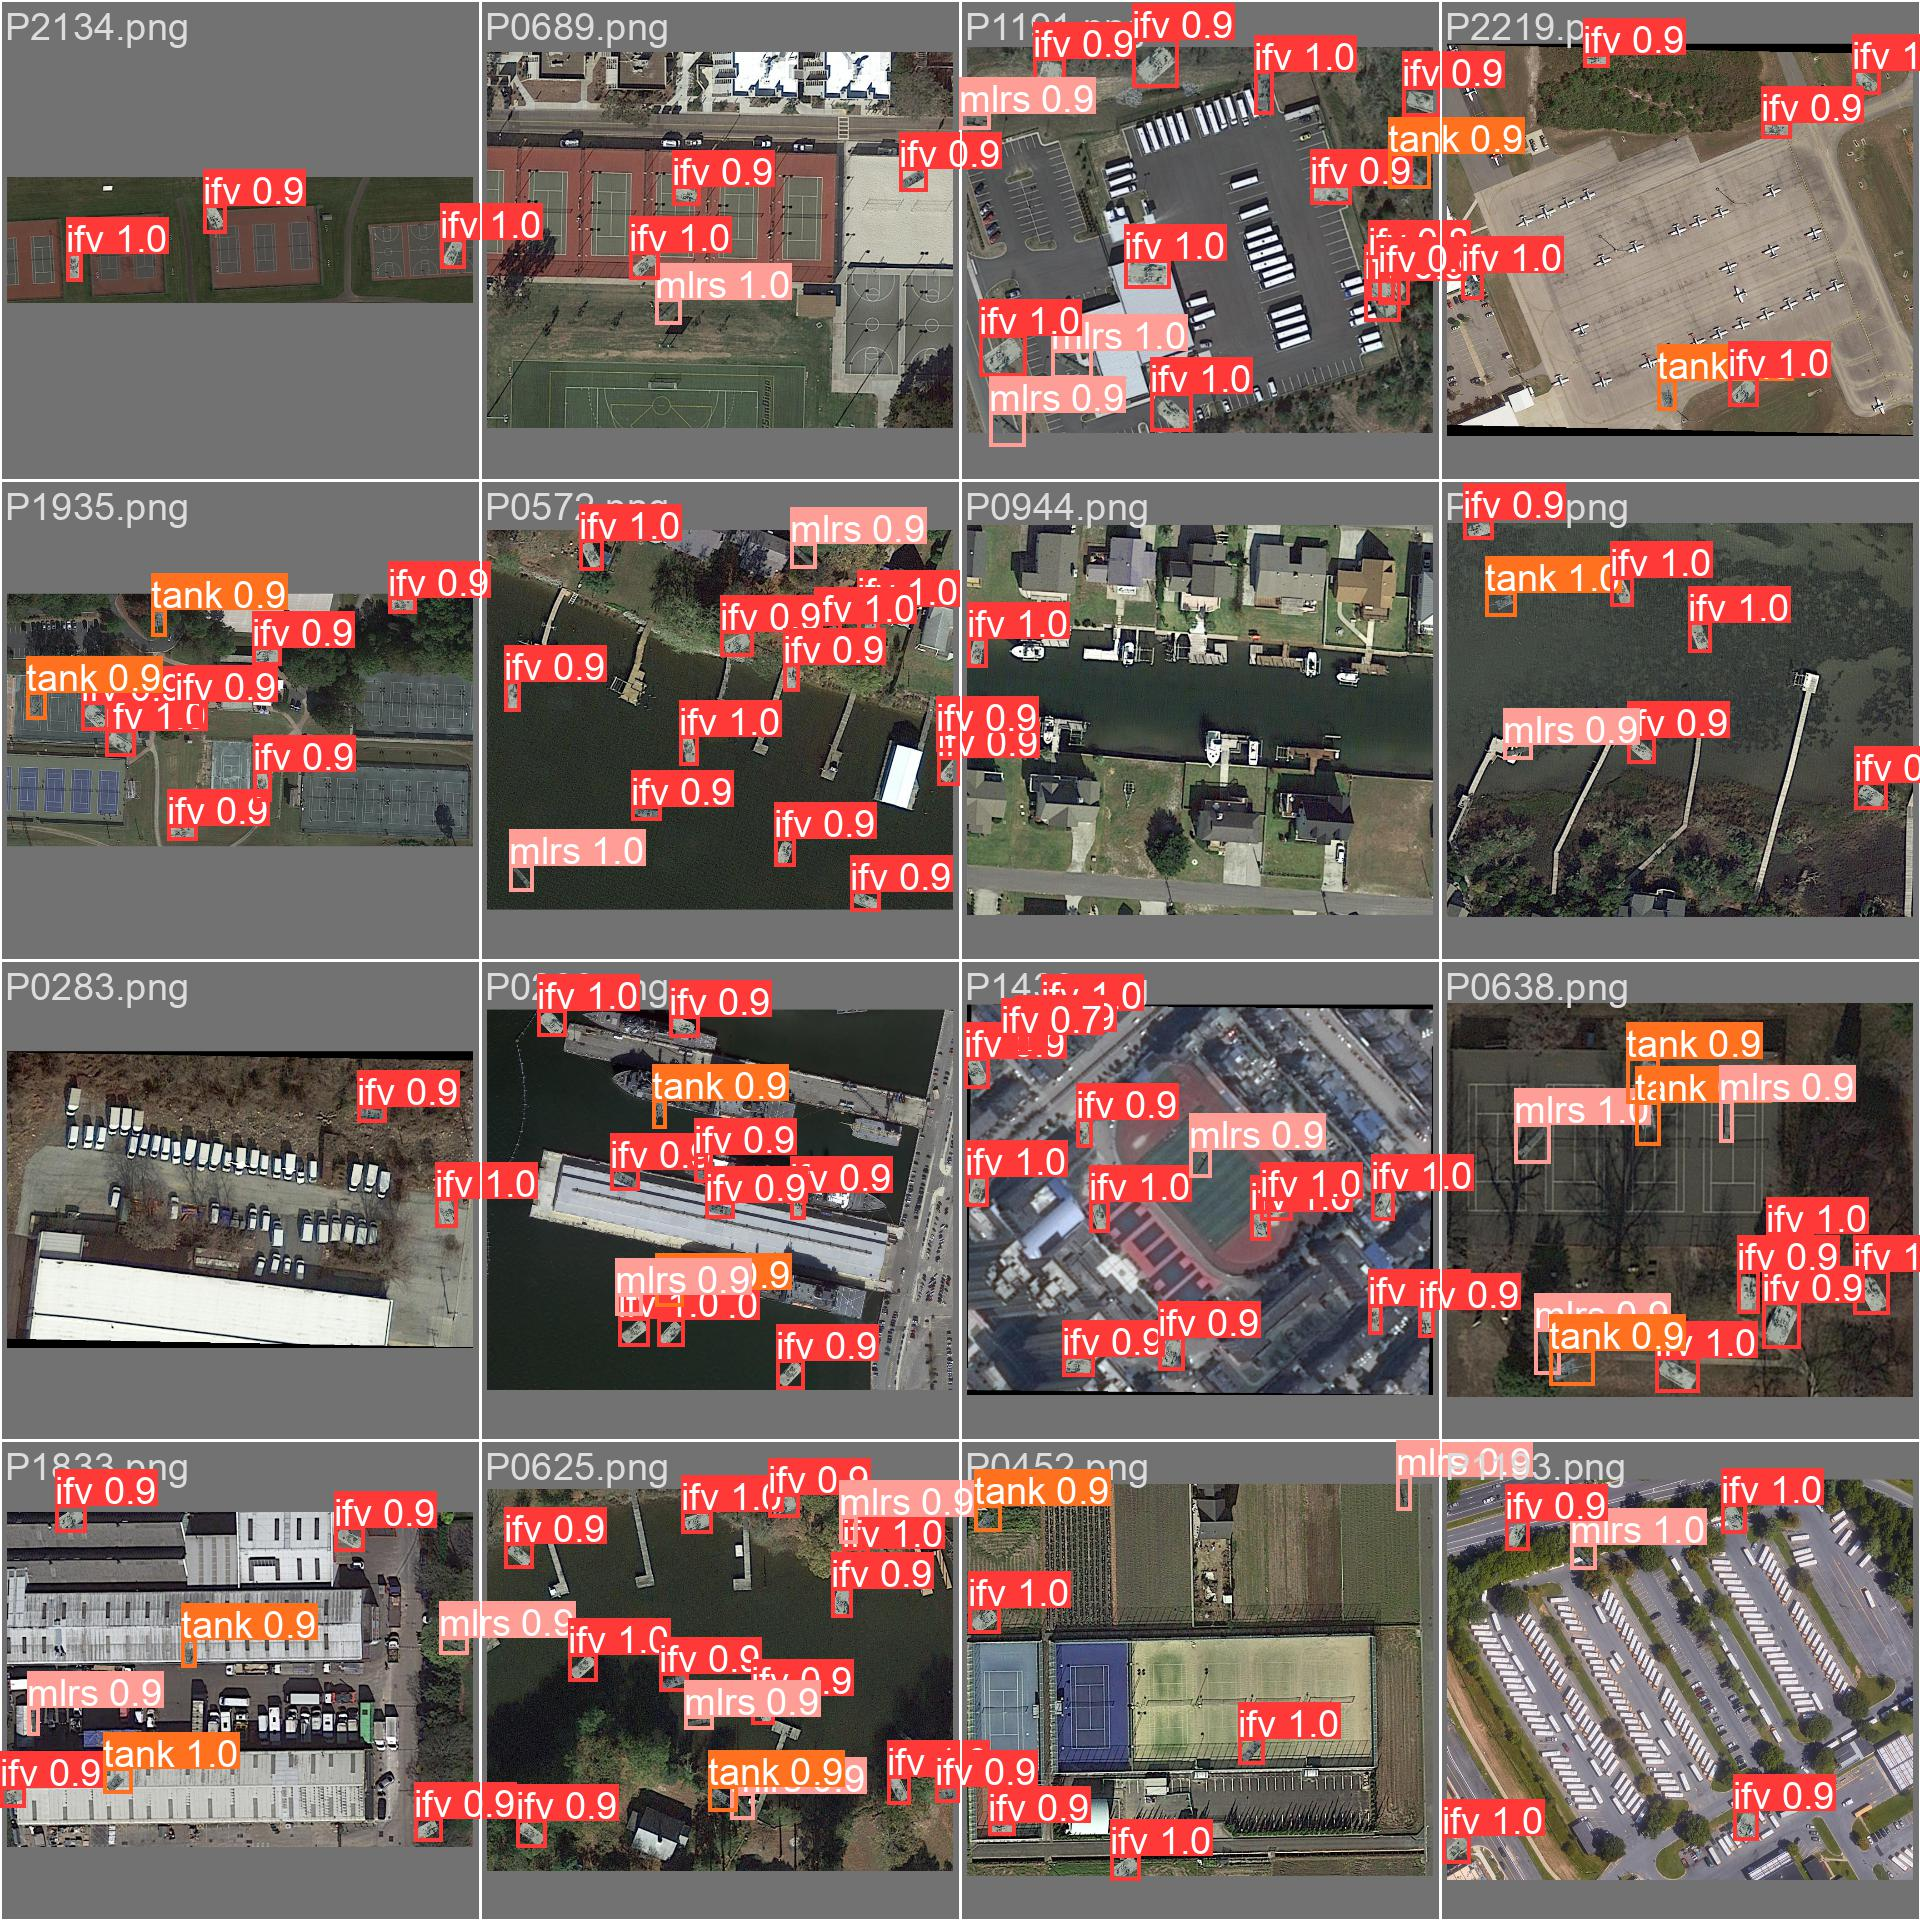
\includegraphics[height=12cm]{images/val-batch0-pred.jpg}
\end{center}


\dod{my-github} TODO content of the GitHub repository
 
\newpage
\thispagestyle{empty}
\addcontentsline{toc}{section}{Bibliography}
\begin{thebibliography}{99}

    \bibitem[10]{map}
    https://towardsdatascience.com/what-is-average-precision-in-object-detection-localization-algorithms-and-how-to-calculate-it-3f330efe697b


    \bibitem[1]{overview}
    Z. Zou, Z. Shi, Y. Guo, J. Ye /
    Object Detection in 20 Years: A Survey. :
    arXiv preprint arXiv:1905.05055 (2019)

    \bibitem[2]{od-overview}
    \textit{Xiaoke Shen} /
    A survey of Object Classification and Detection based on 2D/3D data :
    arXiv preprint arXiv:1905.12683 (2022)

    \bibitem[3]{dog-cat}
    \textit{Great Learning Team} /
    Real-Time Object Detection Using TensorFlow :
    \href{https://www.mygreatlearning.com/blog/object-detection-using-tensorflow/}{mygreatlearning.com}

    \bibitem[4]{my-work-1}
    \textit{Богдан Бугрій} /
    Атаки на глибокі нейронні мережі :
    Львів (2020)

    \bibitem[5]{my-work-2}
    \textit{Богдан Бугрій} /
    Розробка алгоритмів захисту від атак на глибокі нейронні мережі :
    Львів (2021)

    \bibitem[6]{kernel}
    \textit{Axel Thevenot} /
    A visual and mathematical explanation of the 2D convolution layer and its arguments :
    \href{https://towardsdatascience.com/conv2d-to-finally-understand-what-happens-in-the-forward-pass-1bbaafb0b148}{towardsdatascience.com}

    \bibitem[7]{multi-output}    
    \textit{Kaushal Shah} /
    Building Multi Output Cnn With Keras :
    \href{https://kaushal28.github.io/Building-Multi-Output-CNN-with-Keras}{kaushal28.github.io}

    \bibitem[8]{pooling}
    \textit{Jason Brownlee} /
    A Gentle Introduction to Pooling Layers for Convolutional Neural Networks :
    \href{https://machinelearningmastery.com/pooling-layers-for-convolutional-neural-networks}{machinelearningmastery.com}
 

    \bibitem[9]{normalization}
    \textit{Martin Riva} /
    Batch Normalization in Convolutional Neural Networks :
    \href{https://www.baeldung.com/cs/batch-normalization-cnn}{baeldung.com}

    \bibitem[10]{textures}
    \textit{Raitis G.} /
    Battle City tanks repository :
    \href{https://github.com/raitisg/battle-city-tanks}{github.com}

    \bibitem[11]{gradient-descent}
    \textit{Sebastian Ruder} /
    An overview of gradient descent optimization algorithms :
    arXiv preprint arXiv:1609.04747 (2017)

    \bibitem[12]{activations}
    \textit{Johannes Lederer} /
    Activation Functions in Artificial Neural Networks: A Systematic Overview :
    arXiv preprint arXiv:2101.09957 (2021)

    \bibitem[13]{adversarial}
    \textit{Christian Szegedy, Wojciech Zaremba, Ilya Sutskever, Joan Bruna, Dumitru Erhan, Ian Goodfellow, Rob Fergus} /
    Intriguing properties of neural networks :
    arXiv preprint arXiv:1312.6199 (2014)

\end{thebibliography}

\end{document}
